\documentclass[11pt]{article}
\usepackage[utf8]{inputenc}
%\usepackage[latin1]{inputenc}
\usepackage[spanish]{babel}
\decimalpoint
\usepackage{anysize}
\usepackage{graphicx} 
\usepackage{amsmath}
\usepackage{booktabs}
\usepackage{tabulary}
\usepackage{nccmath}
\usepackage{float}
\usepackage{tikz}
\usetikzlibrary{patterns}
\usetikzlibrary{decorations.markings}
\usepackage{pgfplots}
\usepackage{etex}
\usepackage{color}
\usepackage{listings}
\DeclareGraphicsExtensions{.pdf,.png,.jpg}
\renewcommand{\arraystretch}{1.5}
\lstset{ %
language=Python,                % choose the language of the code
basicstyle=\normalsize,       % the size of the fonts that are used for the code
numbers=left,                   % where to put the line-numbers
numberstyle=\footnotesize,      % the size of the fonts that are used for the line-numbers
stepnumber=1,                   % the step between two line-numbers. If it is 1 each line will be numbered
numbersep=5pt,                  % how far the line-numbers are from the code
backgroundcolor=\color{white},  % choose the background color. You must add \usepackage{color}
showspaces=false,               % show spaces adding particular underscores
showstringspaces=false,         % underline spaces within strings
showtabs=false,                 % show tabs within strings adding particular underscores
frame=single,   		% adds a frame around the code
tabsize=4,  		% sets default tabsize to 2 spaces
captionpos=b,   		% sets the caption-position to bottom
breaklines=true,    	% sets automatic line breaking
breakatwhitespace=false,    % sets if automatic breaks should only happen at whitespace
escapeinside={\#}{)}          % if you want to add a comment within your code
}
\marginsize{1.25cm}{1.25cm}{0cm}{2cm}  
\title{Tarea 2 - Operaciones matemáticas básicas - 1a. Parte \\ Curso de Física Computacional}
\author{M. en C. Gustavo Contreras Mayén}
\date{ }
\begin{document}
\maketitle
\fontsize{13}{13}\selectfont
\begin{enumerate}
	\item Dados los puntos
	\begin{table}[H]
		\centering 
		\begin{large}
			\begin{tabulary}{15cm}{c | c | c | c  }\normalsize
				$x$ & $-1.2$ & $0.3$ & $1.1$ \\
				\midrule
				$y$ & $-5.76$ & $-5.61$ & $-3.69$
			\end{tabulary}
		\end{large}
	\end{table}
	Calcula $y$ en $x=0$ usando: a) el método de Neville y b) el método de Lagrange.
	\item Encontrar la raíz de $y(x)$ a partir de los siguientes datos:
	\begin{table}[H]
		\centering 
		\begin{large}
			\begin{tabulary}{15cm}{c | c | c | c | c | c | c | c }
				$x$ & $0$ & $0.5$ & $1$ & $1.5$ & $2$ & $2.5$ & $3$ \\
				\midrule
				$y$ & $1.8421$ & $2.4694$ & $2.4921$ & $1.9047$ & $0.8509$ & $-0.4112$ & $-1.5727$ 
			\end{tabulary}
		\end{large}	
	\end{table}
	Usando la interpolación de Lagrange sobre a) tres puntos, y b) sobre cuatro puntos vecinos más cercanos.
	\item La función $y(x)$ del problema anterior, tiene un máximo en $x=0.7679$. Calcular el valor máximo con el método de interpolación de Neville usando cuatro puntos vecinos.
	\item La viscosidad cinemática $\mu_{k}$ del agua varía con la temperatura $T$ de la siguiente manera:
	\begin{table}[H]
		\centering
			\begin{large} 
				\begin{tabulary}{15cm}{c | c | c | c | c | c | c | c }
					$T(^\circ C)$ & $0$ & $21.1$ & $37.8$ & $54.4$ & $71.1$ & $87.8$ & $100$ \\
					\midrule
					$\mu_{k} (10^{-3}m^{2}/s)$ & $1.79$ & $1.13$ & $0.696$ & $0.519$ & $0.338$ & $0.321$ & $0.296$ 
				\end{tabulary}
			\end{large}
	\end{table}
	Interpolar $\mu_{k}$ para $T= 10^{\circ},30^{\circ},60^{\circ}$ y $90^{\circ}$.
	\item La siguiente tabla muesta como la densidad relativa $\rho$ del aire varía con la altitud $h$. Calcula la densidad relativa del aire en $10.5$ km.
	\begin{table}[H]
		\centering 
		\begin{large}
			\begin{tabulary}{15cm}{c | c | c | c | c | c | c | c }
				$h(km))$ & $0$ & $1.525$ & $3.050$ & $4.575$ & $6.10$ & $7.625$ & $9.150$ \\
				\midrule
				$\rho$ & $1$ & $0.8617$ & $0.7385$ & $0.6292$ & $0.5328$ & $0.4481$ & $0.3741$ 
			\end{tabulary}
		\end{large}
	\end{table}
\newpage
	\item Encuentra todas las raíces positivas de las siguientes ecuaciones mediante el método de bisección, con una tolerancia de 0.001.
	\begin{enumerate}\label{grupo1}
	\renewcommand{\arraystretch}{1.5}
		\item $\tan(x) - x + 1 = 0; \hspace{1cm} 0 < x < 3\pi$
		\item $\sin(x) - 0.3 \exp(x) = 0; \hspace{1cm} x > 0$
		\item $-x^{3} + x + 1 = 0$
		\item $16x^{5} - 20x^{3} + x^{2} + 5x - 0.5 = 0$
	\end{enumerate}
	\item Determina las raíces de las siguientes ecuaciones mediante el método de la falsa posición modificada:
	\begin{enumerate}
		\renewcommand{\arraystretch}{1.5}
		\item $f(x) = 0.5\exp(\frac{x}{3})- \sin(x); \hspace{1cm} x > 0$
		\item $g(x) = \log(1 + x) - x^{2}$
		\item $f(x) = \exp(x) - 5x^{2}$
		\item $h(x) = x^{3} + 2x - 1 = 0$
		\item $f(x) = \sqrt{x+2}$
	\end{enumerate}
	\item Encuentra las raíces de las ecuaciones del problema (\ref{grupo1}) mediante el método de Newton-Raphson, con una tolerancia de $0.0001$
	\item Identifica el intervalo para las raíces de las siguientes ecuaciones y calcula despúes las raíces mediante el método de la secante, con una tolerancia de $0.001$:
	\begin{enumerate}
		\item $0.1 x^{3} - 5 x^{2} - x + 4 + \exp(-x) = 0 $
		\item $\ln(x) -0.2 x^{2} + 1 = 0$
		\item $x + \dfrac{1}{(x+3)x}= 0$
	\end{enumerate}
\item Considera la siguiente imagen:
\begin{figure}[H]
	\centering
	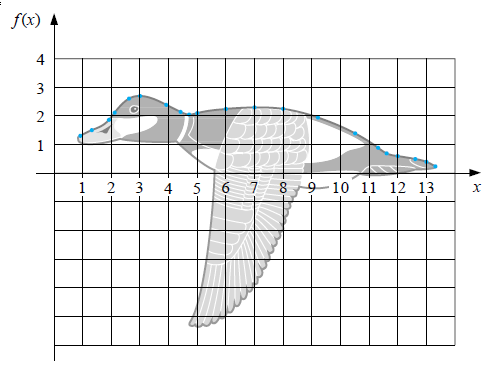
\includegraphics[scale=0.75]{Imagenes/ContornoPato.png} 
\end{figure}
Lo que hay que encontrar es una función que represente el contorno del pato en el primer cuadrante, para ello debes:
\begin{enumerate}
\item Definir un conjunto de puntos (entre 15-20 puntos)
\item Usar la técnica de interpolación de Lagrange para revisar si la función de interpolación, representa debidamente el contorno.
\item Usar la técnica de interpolación con splines.
\end{enumerate}
Discute tus resultados.
\end{enumerate}
\end{document}